% ═══════════════════════════════════════════════════════════════
%  CHAPITRE 2 — TRAVAUX RÉALISÉS
% ═══════════════════════════════════════════════════════════════

\chapter{Travaux R\'ealis\'es : Conception et D\'eveloppement}
\label{chap:travaux_realises}
\vspace{-4pt}
Le chapitre pr\'ec\'edent nous a permis de pr\'esenter notre structure d'accueil et le contexte de notre projet. Ce deuxi\`eme chapitre entre dans le c\oe ur du sujet et d\'ecrit, \'etape par \'etape, le travail effectu\'e. Nous suivrons l'ordre naturel du d\'eveloppement logiciel : analyse des besoins, installation de l'environnement, d\'eveloppement technique, puis r\'esolution des difficult\'es rencontr\'ees.
% ===========================================================
\section{Phase 1 : Analyse des besoins et mod\'elisation}
% ===========================================================
\vspace{-2pt}
Cette phase a consist\'e \`a cerner pr\'ecis\'ement les besoins fonctionnels et techniques du projet, en nous appuyant sur l'observation des plateformes existantes et l'identification des acteurs qui interagiront avec le syst\`eme. L'objectif \'etait de d\'egager les fonctionnalit\'es indispensables avant d'entamer toute activit\'e de d\'eveloppement.
\subsection{\'Etude des solutions existantes}
Nous avons d'abord observ\'e les plateformes immobili\`eres d\'ej\`a utilis\'ees au Cameroun et \`a l'international \hyperref[ref:ownkey_portals]{[4]} (Tableau~\ref{tab:concurrents_existants}). La plupart fonctionnent sur le m\^eme principe : un agent publie manuellement son annonce, et elle reste telle quelle. \`A notre connaissance, ces plateformes ne proposent pas de d\'eduplication entre sources ni de suivi historique des prix ; la quantit\'e d'annonces affich\'ees ne garantit pas non plus la qualit\'e de l'information \hyperref[ref:ownkey_nigeria]{[5]}. D'autres acteurs locaux comme KnF Properties \hyperref[ref:knf]{[6]} compl\`etent ce paysage. C'est ce constat qui a motiv\'e notre travail.
\begin{table}[H]
    \centering
    \footnotesize
    \renewcommand{\arraystretch}{1.4}
    \arrayrulecolor{black}
    \begin{tabularx}{\textwidth}{|l|l|p{2.1cm}|l|X|X|X|}
        \hline
        \rowcolor{headergray}
        \textbf{Nom} & \textbf{Pays} & \textbf{Technologie} & \textbf{Domaine} & \textbf{R\'esultats} & \textbf{Avantages} & \textbf{Limites} \\ \hline
        \textbf{KEUR-IMMO} \hyperref[ref:keurimmo]{[19]} & Int. & Plateforme Web & Immo. & 1\textsuperscript{er} site d'annonces immobili\`eres en Afrique francophone (12 pays, depuis 2022). & Couverture multi-pays, plus de 20 filtres de recherche, audience large. & Saisie manuelle, pas de d\'eduplication entre sources, pas d'historique de prix. \\ \hline
        \textbf{Mapiole} \hyperref[ref:mapiole_app]{[3]} & Cameroun & Application Web, mobile & Annuaire & Acteur local historique avec un fort trafic. & Grand catalogue d'annonces, forte p\'en\'etration locale. & Absence d'historique de prix, aucune d\'eduplication. \\ \hline
        \textbf{Kasastay} & Cameroun & Plateforme Web & Logement & Solution ax\'ee sur la r\'eservation et la location. & Interface moderne, ciblage sp\'ecifique des r\'esidences. & Catalogue restreint, mise \`a jour manuelle des disponibilit\'es. \\ \hline
        \textbf{PUOL} \hyperref[ref:puol]{[20]} & Cameroun & Application Mobile (React Native) & Listing & Application grand public de mise en relation propri\'etaires/locataires. & Acc\`es mobile rapide, recherche simplifi\'ee. & Fonctionnalit\'es limit\'ees, d\'ependance du r\'eseau mobile, pas d'historique de prix. \\ \hline
        \textbf{Ny\`e Ta Piole} \hyperref[ref:nyetapiole]{[21]} & Cameroun & Plateforme Web temps r\'eel & Proptech & Proptech \'emergente connectant directement propri\'etaires et locataires. & Contact direct sans interm\'ediaire, co\^ut de mise en relation inf\'erieur \`a 500 FCFA. & Catalogue restreint, pas de cartographie avanc\'ee, pas d'historique de prix. \\ \hline
    \end{tabularx}
    \caption{Comparaison des solutions existantes sur le march\'e immobilier}
    \label{tab:concurrents_existants}
\end{table}
\vspace{-6pt}
\subsection{Acteurs du syst\`eme}
Le diagramme de cas d'utilisation (\textbf{Figure~\ref{fig:use_case}}) identifie deux types d'utilisateurs. \textbf{L'utilisateur final} cherche un logement : il filtre les annonces, compare les prix entre plateformes, ou affiche sur une carte les maisons accessibles en moins de X minutes depuis son travail. \textbf{L'administrateur} g\`ere le syst\`eme en arri\`ere-plan : il lance les robots de collecte et valide manuellement les annonces en cas de doute.
% ==============================================================
%  DIAGRAMME — Cas d'utilisation de la plateforme
%  Fichier externe, appelé via \input dans le chapitre 2
% ==============================================================
\begin{figure}[H]
\centering
\begin{tikzpicture}[node distance=5mm and 2.5cm, scale=0.85, every node/.style={scale=0.85}]
  % --- Titre ---
  \node[align=center, font=\small\bfseries\sffamily, text=ciGreen, text width=8cm] (titleNode) {SERVICES DE L'APPLICATION};

  % --- Pile verticale des Use Cases ---
  \node[node-green, below=6mm of titleNode, text width=4.5cm] (uc1) {Rechercher par filtres};
  \node[node-green, below=of uc1, text width=4.5cm] (uc2) {Comparer les prix des sources};
  \node[node-green, below=of uc2, text width=4.5cm] (uc3) {Recherche par temps de trajet};
  \node[node-green, below=of uc3, text width=4.5cm] (uc4) {Consulter les tendances prix par quartier};
  \node[node-gold, below=of uc4, text width=4.5cm] (uc5) {Mod\'erer les anomalies};
  \node[node-gold, below=of uc5, text width=4.5cm] (uc6) {D\'eclencher/Surveiller crawls};

  % --- Acteur Gauche (Utilisateur Final) ---
  \node[align=center, left=2.5cm of uc2.south west] (user) {
    \begin{tikzpicture}[scale=0.4]
      \draw[fill=white, line width=0.8pt] (0,1) circle (0.25);
      \draw[line width=0.8pt] (0,0.75) -- (0,0);
      \draw[line width=0.8pt] (-0.35,0.45) -- (0.35,0.45);
      \draw[line width=0.8pt] (0,0) -- (-0.25,-0.5);
      \draw[line width=0.8pt] (0,0) -- (0.25,-0.5);
    \end{tikzpicture}\\
    \small Utilisateur Final
  };

  % --- Acteur Droite (Administrateur) ---
  \node[align=center, right=2.5cm of uc5.north east] (admin) {
    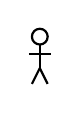
\begin{tikzpicture}[scale=0.4]
      \draw[fill=white, line width=0.8pt] (0,1) circle (0.25);
      \draw[line width=0.8pt] (0,0.75) -- (0,0);
      \draw[line width=0.8pt] (-0.35,0.45) -- (0.35,0.45);
      \draw[line width=0.8pt] (0,0) -- (-0.25,-0.5);
      \draw[line width=0.8pt] (0,0) -- (0.25,-0.5);
    \end{tikzpicture}\\
    \small Administrateur /\\Crawler
  };

  % Frontière du système
  \begin{scope}[on background layer]
    \node[group-box, fit=(titleNode) (uc1) (uc2) (uc3) (uc4) (uc5) (uc6), inner xsep=0.4cm, inner ysep=0.4cm] (system-boundary) {};
  \end{scope}

  % Connecteurs de l'Utilisateur Final
  \draw[flow-arrow] (user.east) -- (uc1.west);
  \draw[flow-arrow] (user.east) -- (uc2.west);
  \draw[flow-arrow] (user.east) -- (uc3.west);
  \draw[flow-arrow] (user.east) -- (uc4.west);

  % Connecteurs de l'Administrateur
  \draw[flow-arrow-gold] (admin.west) -- (uc5.east);
  \draw[flow-arrow-gold] (admin.west) -- (uc6.east);
\end{tikzpicture}
\caption{Diagramme de cas d'utilisation de la plateforme}
\label{fig:use_case}
\end{figure}
\vspace{-4pt}
\subsection{Besoins fonctionnels et non fonctionnels}
Le tableau~\ref{tab:besoins} r\'esume les besoins identifi\'es lors de cette phase d'analyse.
\begin{table}[H]
    \centering
    \small
    \renewcommand{\arraystretch}{1.3}
    \begin{tabularx}{\textwidth}{|l|X|X|}
        \hline
        \rowcolor{headergray}
        \textbf{Cat\'egorie} & \textbf{Besoin} & \textbf{Description} \\ \hline
        \multirow{4}{*}{\textbf{Fonctionnels}}
        & Collecte automatique & Extraire p\'eriodiquement les annonces depuis plusieurs sites sans intervention humaine. \\ \cline{2-3}
        & D\'eduplication & D\'etecter quand une m\^eme maison appara\^it sur plusieurs plateformes et cr\'eer une fiche unique (Super-Annonce). \\ \cline{2-3}
        & Historique des prix & Conserver chaque changement de prix constat\'e au fil du temps. \\ \cline{2-3}
        & Interface mobile et web & Proposer une application avec carte, recherche avanc\'ee et assistant IA. \\ \hline
        \multirow{3}{*}{\textbf{Non fonctionnels}}
        & Performance & L'application doit rester fluide m\^eme avec des milliers d'annonces en base. \\ \cline{2-3}
        & Fiabilit\'e & Les robots de collecte ne doivent pas planter si un site est temporairement indisponible. \\ \cline{2-3}
        & S\'ecurit\'e & L'acc\`es aux fonctions d'administration doit \^etre prot\'eg\'e par cl\'e d'authentification. \\ \hline
    \end{tabularx}
    \caption{Synth\`ese des besoins fonctionnels et non fonctionnels}
    \label{tab:besoins}
\end{table}
% ===========================================================
% ===========================================================
\vspace{-6pt}
\section{Phase 2 : Installation et configuration de l'environnement}
% ===========================================================
\vspace{-2pt}
Avant d'installer nos outils de travail, nous avons d\^u faire des choix technologiques. Nous avons compar\'e plusieurs options pour le serveur, la base de donn\'ees et l'application mobile afin de retenir les solutions les mieux adapt\'ees \`a nos besoins.

\textbf{1. Choix du serveur (Backend)}
\vspace{-6pt}
\begin{table}[H]
    \centering
    \footnotesize
    \renewcommand{\arraystretch}{1.2}
    \begin{tabularx}{\textwidth}{|l|c|X|c|}
        \hline
        \rowcolor{headergray}
        \textbf{Technologie} & \textbf{Vitesse} & \textbf{Justification / Limites} & \textbf{Choix} \\ \hline
        \textbf{Django} & Moyenne & Assez lourd \`a configurer, peu adapt\'e au traitement temps r\'eel. & Non \\ \hline
        \textbf{Node.js} & Rapide & Manque de v\'erification stricte des types de donn\'ees. & Non \\ \hline
        \textbf{FastAPI} \hyperref[ref:fastapi]{[9]} & Tr\`es rapide & \textbf{Adopt\'e pour sa vitesse et sa simplicit\'e \`a g\'erer la collecte en continu.} & \textbf{Oui} \\ \hline
    \end{tabularx}
\end{table}

\vspace{-12pt}
\textbf{2. Choix de la base de donn\'ees}
\vspace{-6pt}
\begin{table}[H]
    \centering
    \footnotesize
    \renewcommand{\arraystretch}{1.2}
    \begin{tabularx}{\textwidth}{|l|c|X|c|}
        \hline
        \rowcolor{headergray}
        \textbf{Technologie} & \textbf{S\'ecurit\'e} & \textbf{Justification / Limites} & \textbf{Choix} \\ \hline
        \textbf{MongoDB} & Faible & Base non relationnelle (NoSQL), difficile d'y relier des annonces entre elles. & Non \\ \hline
        \textbf{MySQL} & Bonne & Un peu moins performant pour la recherche g\'eographique sur carte. & Non \\ \hline
        \textbf{PostgreSQL} \hyperref[ref:postgresql]{[16]} & Excellente & \textbf{Adopt\'e pour sa gestion de la cartographie, de la recherche plein texte \hyperref[ref:postgres_es]{[11]} et de l'historique.} & \textbf{Oui} \\ \hline
    \end{tabularx}
\end{table}

\vspace{-12pt}
\textbf{3. Choix de l'application mobile}
\vspace{-6pt}
\begin{table}[H]
    \centering
    \footnotesize
    \renewcommand{\arraystretch}{1.2}
    \begin{tabularx}{\textwidth}{|l|c|X|c|}
        \hline
        \rowcolor{headergray}
        \textbf{Technologie} & \textbf{Fluidit\'e} & \textbf{Justification / Limites} & \textbf{Choix} \\ \hline
        \textbf{React Native} & Moyenne & Risque de lenteur ou de bugs sur l'affichage de notre carte interactive. & Non \\ \hline
        \textbf{Android Java} & Tr\`es bonne & Ne fonctionne que sur Android, ce qui exclurait les utilisateurs d'iPhone. & Non \\ \hline
        \textbf{Flutter} \hyperref[ref:flutter]{[10]} & Tr\`es bonne & \textbf{Adopt\'e car il est fluide et cr\'ee les versions Android et iOS en m\^eme temps.} & \textbf{Oui} \\ \hline
    \end{tabularx}
\end{table}
\vspace{-4pt}

Suite \`a ces d\'ecisions, nous avons install\'e Python/FastAPI, isol\'e notre base PostgreSQL gr\^ace \`a l'outil de virtualisation Docker \hyperref[ref:docker]{[12]} (pour garantir la m\^eme configuration entre coll\`egues), et install\'e le SDK Flutter sous Android Studio. Ces d\'eveloppements reposent sur l'architecture pr\'esent\'ee \`a la \textbf{Figure~\ref{fig:archi_generale}} : les robots d'extraction en haut, le serveur et la base de donn\'ees au centre, et l'application client en bas.

% ==============================================================
%  DIAGRAMME — Architecture globale multi-couche CentralImmo
%  Fichier externe, appelé via \input dans le chapitre 2
% ==============================================================
\begin{figure}[H]
\centering
\begin{tikzpicture}[node distance=8mm and 8mm, scale=0.9, every node/.style={scale=0.9}]
  % --- Plan Collecte (Scrapers) ---
  \node[node-gold] (mapiole) {Scraper D\'edi\'e\\Mapiole (Python)};
  \node[node-gold, right=8mm of mapiole] (kasastay) {Scraper D\'edi\'e\\Kasastay (Python)};
  \node[node-gold, right=8mm of kasastay] (universal) {Scraper Universel\\(Heuristiques)};
  % --- Plan API (FastAPI) ---
  \node[node-green, below=15mm of kasastay, text width=6cm] (fastapi) {
    \textbf{Serveur Backend (FastAPI)}\\
    \footnotesize
    $\bullet$ Ingestion \& d\'eduplication (DCS)\\
    $\bullet$ API de recherche naturelle \& isochrone
  };
  % --- Plan Persistance (Base de données) ---
  \node[node-white, right=12mm of fastapi, text width=4.5cm] (db) {
    \textbf{Base PostgreSQL}\\
    \color{ciDark}\scriptsize
    $\bullet$ \texttt{raw\_listings}\\
    $\bullet$ \texttt{canonical\_properties}\\
    $\bullet$ \texttt{listing\_history}\\
    $\bullet$ \texttt{locations}
  };
  % --- Plan Présentation (Flutter) ---
  \node[node-blue, below=15mm of fastapi, text width=5cm] (client) {
    \textbf{Application Mobile (Flutter)}\\
    \footnotesize Interface unifi\'ee Trivago-style
  };
  % --- Groupes ---
  \begin{scope}[on background layer]
    \node[group-box, fit=(mapiole) (kasastay) (universal), label={[font=\footnotesize\bfseries\sffamily, text=ciGold!80!black]above:1. PHASE DE COLLECTE ET EXTRACTION}] (box-collecte) {};
  \end{scope}
  % --- Liaisons ---
  \draw[flow-arrow] (mapiole.south) -- ++(0,-4mm) -| ([xshift=-1.5cm]fastapi.north);
  \draw[flow-arrow] (kasastay.south) -- (fastapi.north);
  \draw[flow-arrow] (universal.south) -- ++(0,-4mm) -| ([xshift=1.5cm]fastapi.north);
  \draw[<->, line width=1.1pt, draw=ciGreen] (fastapi) -- node[label-style, above] {SQL} (db);
  \draw[<->, line width=1.1pt, draw=ciBlue] (client) -- node[label-style, right] {HTTP/REST} (fastapi);
\end{tikzpicture}
\caption{Architecture globale multi-couche de CentralImmo}
\label{fig:archi_generale}
\end{figure}

% ===========================================================
\vspace{-4pt}
\section{Phase 3 : D\'eveloppement du logiciel}
% ===========================================================
\vspace{-2pt}
C'est la partie o\`u nous avons pass\'e le plus de temps. Nous avons d\'evelopp\'e le logiciel brique par brique.
\subsection{Construction de la base de donn\'ees}
L'id\'ee principale \'etait de s\'eparer trois niveaux d'information (\textbf{Figure~\ref{fig:mcd_db}}) : (1)~les \textbf{annonces brutes} (\texttt{RawListings}), o\`u tout ce que le syst\`eme r\'ecup\`ere sur internet est stock\'e sans modification pour garder la trace de l'origine ; (2)~les \textbf{fiches unifi\'ees} (\texttt{CanonicalProperties}), o\`u les annonces brutes d\'ecrivant la m\^eme maison sont regroup\'ees en une "Super-Annonce" visible sur le mobile ; (3)~\textbf{l'historique des prix} (\texttt{ListingHistory}), o\`u chaque changement de prix est enregistr\'e sans effacer l'ancien, permettant de suivre l'\'evolution des tarifs.
% ==============================================================
%  DIAGRAMME — Modèle Conceptuel des Données (MCD) multi-calques
%  Fichier externe, appelé via \input dans le chapitre 2
% ==============================================================
\begin{figure}[H]
\centering
\begin{tikzpicture}[node distance=1.2cm and 1.8cm, scale=0.85, every node/.style={scale=0.85}]
  % Entité Source
  \node[node-gold, text width=4.2cm] (src) {
    \textbf{Entity: Sources}\\
    \color{ciGreen}\scriptsize PK: id (integer)\\
    \color{ciDark}\tiny
    $\bullet$ slug (unique string)\\
    $\bullet$ display\_name (string)\\
    $\bullet$ adapter\_kind (string)
  };
  % Entité RawListing
  \node[node-green, below=of src, text width=4.2cm] (raw) {
    \textbf{Entity: RawListings}\\
    \color{ciGreen}\scriptsize PK: id (bigint)\\
    \color{ciDark}\tiny
    $\bullet$ url\_source (text)\\
    $\bullet$ url\_hash (unique)\\
    $\bullet$ title\_raw (string)\\
    $\bullet$ price\_parsed (bigint)\\
    \color{ciBlue}FK: source\_id\\
    \color{ciBlue}FK: canonical\_property\_id
  };
  % Entité CanonicalProperty
  \node[node-green, right=of raw, text width=4.5cm] (canon) {
    \textbf{Entity: CanonicalProperties}\\
    \color{ciGreen}\scriptsize PK: id (bigint)\\
    \color{ciDark}\tiny
    $\bullet$ match\_key (string)\\
    $\bullet$ title\_canonical (string)\\
    $\bullet$ current\_best\_price (bigint)\\
    \color{ciBlue}FK: location\_id
  };
  % Entité Location
  \node[node-white, above=of canon, text width=4.2cm] (loc) {
    \textbf{Entity: Locations}\\
    \color{ciGreen}\scriptsize PK: id (bigint)\\
    \color{ciDark}\tiny
    $\bullet$ city (string)\\
    $\bullet$ neighborhood (string)\\
    $\bullet$ slug (string)
  };
  % Entité ListingHistory
  \node[node-red, right=of canon, text width=4.2cm] (hist) {
    \textbf{Entity: ListingHistory}\\
    \color{ciGreen}\scriptsize PK: id (bigint)\\
    \color{ciDark}\tiny
    $\bullet$ event\_type (string)\\
    $\bullet$ price\_observed (bigint)\\
    $\bullet$ observed\_at (datetime)
  };
  % Relations
  \draw[flow-arrow, draw=ciGold] (src.south) -- node[label-style, left] {1..N} (raw.north);
  \draw[flow-arrow, draw=ciGreen] (raw.east) -- node[label-style, above] {N..0-1} (canon.west);
  \draw[flow-arrow, draw=ciGreen] (loc.south) -- node[label-style, right] {1..N} (canon.north);
  \draw[flow-arrow, draw=ciRed] (canon.east) -- node[label-style, above] {1..N} (hist.west);
  \draw[flow-arrow, draw=ciRed, bend right=20] (raw.south) -- ++(0,-0.5cm) -| node[label-style, pos=0.3, below] {1..N} (hist.south);
\end{tikzpicture}
\caption{Mod\`ele Conceptuel des Donn\'ees multi-calques (MCD)}
\label{fig:mcd_db}
\end{figure}
\vspace{-4pt}
\subsection{Les robots de collecte (Web Scraping)}
Nous avons d\'evelopp\'e en Python des programmes appel\'es \emph{crawlers}, reposant sur la biblioth\`eque BeautifulSoup \hyperref[ref:beautifulsoup]{[13]}, qui se connectent aux sites d'annonces, lisent les pages et en extraient les informations utiles (titre, prix, localisation, photos). Comme le montre la \textbf{Figure~\ref{fig:ingest_pipeline}}, quand un crawler envoie une annonce au serveur, celui-ci v\'erifie d'abord si le lien de cette annonce existe d\'ej\`a en base. Si oui, il met simplement \`a jour la date et note le prix actuel. Si non, c'est une nouvelle annonce qui entre dans le circuit de traitement. Ce m\'ecanisme, appel\'e idempotence, \'evite de cr\'eer des doublons dans notre propre base.
% ==============================================================
%  DIAGRAMME — Pipeline d'ingestion et d'idempotence
%  Fichier externe, appelé via \input dans le chapitre 2
% ==============================================================
\begin{figure}[H]
\centering
\begin{tikzpicture}[node distance=8mm, scale=0.88, every node/.style={scale=0.88}]
  \node[node-gold] (start) {Donn\'ees extraites brutes\\(\texttt{RawListingDraft})};
  \node[base-node, draw=ciDark, shape=diamond, aspect=2.2, below=6mm of start] (dec1) {L'URL existe en base ?};
  % --- Branche Gauche (Re-crawl) ---
  \node[node-white, left=1cm of dec1, text width=3.6cm] (recrawl) {\textbf{D\'ej\`a archiv\'ee}\\Mise \`a jour \texttt{last\_seen\_at}};
  \node[base-node, draw=ciDark, shape=diamond, aspect=2.2, below=6mm of recrawl] (dec2) {Le prix a chang\'e ?};
  \node[node-green, below=6mm of dec2, text width=3.6cm] (hist-price) {Ajout d'un point de prix dans \texttt{listing\_history}};
  % --- Branche Droite (Nouveau) ---
  \node[node-white, right=1cm of dec1, text width=3.6cm] (new) {\textbf{Inconnu}\\R\'esolution adresse et g\'eographie};
  \node[node-green, below=8mm of new, text width=3.6cm] (match) {Traitement de d\'eduplication DCS};
  \node[node-blue, below=8mm of match, text width=3.6cm] (insert) {Insertion PostgreSQL \& Liaisons};

  \draw[flow-arrow] (start) -- (dec1);
  \draw[flow-arrow] (dec1.west) -- node[label-style, above] {Oui} (recrawl.east);
  \draw[flow-arrow] (dec1.east) -- node[label-style, above] {Non} (new.west);
  \draw[flow-arrow] (recrawl) -- (dec2);
  \draw[flow-arrow] (dec2.south) -- node[label-style, right] {Oui} (hist-price.north);
  \draw[flow-arrow] (dec2.west) -- node[label-style, above] {Non} ++(-1cm, 0) |- (hist-price.west);
  \draw[flow-arrow] (new) -- (match);
  \draw[flow-arrow] (match) -- (insert);
\end{tikzpicture}
\caption{Algorithme d\'ecisionnel du pipeline d'ingestion de CentralImmo}
\label{fig:ingest_pipeline}
\end{figure}
\vspace{-4pt}
\subsection{L'algorithme de d\'eduplication (DCS)}
Le DCS (\emph{Duplicate Confidence Score}) est l'algorithme que nous avons con\c{c}u pour d\'eterminer si deux annonces, venant de deux sites diff\'erents, parlent de la m\^eme maison. Il compare quatre crit\`eres et attribue une note sur 100 (\textbf{Figure~\ref{fig:arbre_dcs}}) : la ressemblance des titres, la proximit\'e des prix (\'ecart inf\'erieur \`a 15\,\%), le type de bien (studio, villa, duplex), et le nombre de chambres.
% ==============================================================
%  DIAGRAMME — Arbre de décision DCS (Duplicate Confidence Score)
%  Fichier externe, appelé via \input dans le chapitre 2
% ==============================================================
\begin{figure}[H]
\centering
\begin{tikzpicture}[
  node distance=4mm and 1cm,
  font=\scriptsize\sffamily,
  >=Stealth,
  factorNode/.style={
    draw=ciBorder, line width=0.8pt, rounded corners=3pt,
    fill=white, text=ciDark, align=center,
    text width=3.8cm, inner sep=5pt
  },
  weightNode/.style={
    draw=ciGold!80!black, line width=0.8pt, rounded corners=3pt,
    fill=ciGoldLight, text=ciDark, align=center,
    text width=2.2cm, inner sep=5pt
  },
  sumNode/.style={
    draw=ciGreen, line width=0.9pt, rounded corners=3pt,
    fill=ciGreenLight, text=ciDark, align=center,
    text width=2.2cm, inner sep=6pt
  },
  decisionGreen/.style={
    draw=ciGreen, line width=0.8pt, rounded corners=3pt,
    fill=ciGreenLight, text=ciDark, align=center,
    text width=2.6cm, inner sep=5pt
  },
  decisionGold/.style={
    draw=ciGold!80!black, line width=0.8pt, rounded corners=3pt,
    fill=ciGoldLight, text=ciDark, align=center,
    text width=2.6cm, inner sep=5pt
  },
  decisionRed/.style={
    draw=ciRed, line width=0.8pt, rounded corners=3pt,
    fill=ciRed!8, text=ciDark, align=center,
    text width=2.6cm, inner sep=5pt
  },
  arrow/.style={-Stealth, line width=0.8pt},
  arrowGold/.style={-Stealth, line width=0.8pt, draw=ciGold!80!black},
  arrowGreen/.style={-Stealth, line width=0.8pt, draw=ciGreen},
  arrowRed/.style={-Stealth, line width=0.8pt, draw=ciRed}
]

  % --- Colonnes : Facteurs | Poids | Somme | Décisions ---

  % Facteurs (colonne gauche)
  \node[factorNode] (f1) {Similitude de Titre\\(RapidFuzz)};
  \node[factorNode, below=of f1] (f2) {Proximit\'e de Prix\\(\'ecart $<$ 15\,\%)};
  \node[factorNode, below=of f2] (f3) {Type de bien\\(Villa, Studio, \ldots)};
  \node[factorNode, below=of f3] (f4) {Nombre de chambres\\(comparaison exacte)};

  % Poids (colonne milieu-gauche)
  \node[weightNode, right=1cm of f1] (p1) {Poids : 35\,\%};
  \node[weightNode, right=1cm of f2] (p2) {Poids : 25\,\%};
  \node[weightNode, right=1cm of f3] (p3) {Poids : 20\,\%};
  \node[weightNode, right=1cm of f4] (p4) {Poids : 20\,\%};

  % Somme pondérée (colonne centre)
  \node[sumNode, right=1.4cm of p2, yshift=-4.5mm, minimum height=1.6cm] (sum)
    {\textbf{Somme\\Pond\'er\'ee}\\[2pt]\scriptsize Score / 100};

  % Décisions (colonne droite)
  \node[decisionGreen, right=1.4cm of sum, yshift=1.3cm] (conf)
    {\textbf{Fiche Fusionn\'ee}\\Score $\geq$ 85\,\%};
  \node[decisionGold, right=1.4cm of sum] (prob)
    {\textbf{Validation manuelle}\\65\,\% -- 84\,\%};
  \node[decisionRed, right=1.4cm of sum, yshift=-1.3cm] (newp)
    {\textbf{Nouveau Bien}\\Score $<$ 65\,\%};

  % --- Flèches : Facteurs -> Poids -> Somme ---
  \draw[arrow] (f1) -- (p1);
  \draw[arrow] (f2) -- (p2);
  \draw[arrow] (f3) -- (p3);
  \draw[arrow] (f4) -- (p4);

  \draw[arrowGold] (p1.east) -- (sum.north west);
  \draw[arrowGold] (p2.east) -- (sum.west);
  \draw[arrowGold] (p3.east) -- (sum.west);
  \draw[arrowGold] (p4.east) -- (sum.south west);

  % --- Flèches : Somme -> Décisions ---
  \draw[arrowGreen] (sum.east) -- (conf.west);
  \draw[arrowGold]  (sum.east) -- (prob.west);
  \draw[arrowRed]   (sum.east) -- (newp.west);

\end{tikzpicture}
\caption{Algorithme de d\'ecision sur la d\'eduplication DCS}
\label{fig:arbre_dcs}
\end{figure}
\vspace{-2pt}
Si le score d\'epasse 85\,\%, les annonces sont fusionn\'ees automatiquement. Entre 65\,\% et 84\,\%, l'annonce est mise en attente pour validation manuelle par l'administrateur. En dessous de 65\,\%, ce sont deux biens distincts. La comparaison textuelle utilise la biblioth\`eque \textbf{RapidFuzz} \hyperref[ref:rapidfuzz]{[14]}, \'ecrite en C++, qui permet des comparaisons rapides m\^eme sur un volume important d'annonces.
\subsection{L'application mobile (Flutter)}
L'interface s'inspire du mod\`ele Trivago : l'\'ecran principal affiche des fiches propres (Super-Annonces) sans indiquer de quelle plateforme elles proviennent, pour ne pas influencer l'utilisateur. La page de d\'etail permet ensuite de comparer les prix propos\'es par chaque source, avec les liens directs vers chacune. L'application int\`egre \'egalement une carte qui affiche les maisons accessibles en moins de X minutes depuis un point choisi (fonction isochrone), ainsi qu'un assistant IA qui permet de chercher un bien en langage naturel.
% ===========================================================
\section{Phase 4 : Difficult\'es rencontr\'ees et solutions}
% ===========================================================
\vspace{-2pt}
Comme dans tout projet, nous avons rencontr\'e des difficult\'es techniques en cours de route. Le tableau~\ref{tab:difficultes} r\'esume les principaux probl\`emes et les solutions apport\'ees.
\begin{table}[H]
    \centering
    \small
    \renewcommand{\arraystretch}{1.4}
    \arrayrulecolor{black}
    \begin{tabularx}{\textwidth}{|p{4.5cm}|X|}
        \hline
        \rowcolor{headergray}
        \textbf{Difficult\'e rencontr\'ee} & \textbf{Solution apport\'ee} \\ \hline
        H\'et\'erog\'en\'eit\'e des sites sources : chaque site affichait ses annonces selon une structure HTML et une mise en forme diff\'erentes. & Analyse approfondie des diff\'erents sites, un par un, afin d'identifier et de mod\'eliser les patterns sp\'ecifiques \`a chaque source avant d'\'ecrire les extracteurs correspondants. \\ \hline
        Lenteur de l'algorithme de d\'eduplication : chaque nouvelle annonce \'etait compar\'ee \`a toutes celles d\'ej\`a en base. & Pr\'e-filtrage par quartier et type de bien (un studio \`a Mvan n'est jamais compar\'e \`a une villa \`a Bastos), \'eliminant environ 95\,\% des comparaisons inutiles. \\ \hline
    \end{tabularx}
    \caption{Synth\`ese des difficult\'es rencontr\'ees et des solutions adopt\'ees}
    \label{tab:difficultes}
\end{table}
\paragraph*{Conclusion du chapitre}
Ce chapitre a pr\'esent\'e le travail r\'ealis\'e durant notre stage en suivant les grandes phases du d\'eveloppement logiciel : analyse, installation, d\'eveloppement et r\'esolution des difficult\'es. Nous avons construit une base de donn\'ees multi-calques, des robots de collecte, un algorithme de d\'eduplication et une application mobile et web. Le chapitre suivant dressera le bilan des r\'esultats obtenus et proposera une r\'eflexion sur les comp\'etences acquises.
